\documentclass[11 pt,russian]{article}
\hoffset=-2cm \voffset=-2.5cm \textwidth=17cm \textheight=23cm

\usepackage[utf8]{inputenc}
\usepackage[russian]{babel}
\usepackage{amssymb, amsfonts, amsthm, amsmath}
\usepackage{graphicx}
\DeclareGraphicsRule{*}{mps}{*}{}

\newcounter{variant}
\newcounter{zadacha}[variant]

\newcommand{\z}{\par\addtocounter{zadacha}{1}%
\textbf{\Roman{zadacha}}\ }

%=============================================

\begin{document}
№7\\
$|x-7|+|x-5|=x-4$\\
Построим на числовой оси знаки раскрытия модулей в зависимости от $x$\\\\
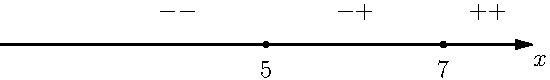
\includegraphics[scale =1]{7.pdf}\\
\setcounter{zadacha}{0}
\z случай\\
$x\leqslant5$\\
$-x+7-x+5=x-4$\\
$-3x=-16$\\
$x=\dfrac{16}3$\\
$\dfrac{16}3>5 \Rightarrow \dfrac{16}3 - \text{не подходит.}$
\z случай\\
$5<x<7$\\
$-x+7+x-5=x-4$\\
$x=6$\\
$5<6<7 \Rightarrow x=6 - \text{походит.}$
\z случай\\
$x\geqslant 7$\\
$x-7+x-5=x-4$\\
$x=8$\\
$8\geqslant7 \Rightarrow x=8 - \text{подходит.}$\\
Ответ: \{6,8\}.
\end{document}